\chapter{Estado del arte y marco tecnológico}
\label{ch:estadoarte}

\section{Fundamentos y enfoques}

La movilidad urbana se ha consolidado como un ámbito de estudio en el que confluyen la ingeniería del transporte, la analítica de datos y la inteligencia artificial. En este contexto, los simuladores actuales no se limitan a representar mapas o a calcular rutas aisladas, sino que actúan como herramientas para evaluar políticas y escenarios de movilidad, permitiendo analizar de forma anticipada cómo cambios en los costes, en la oferta de transporte o en las condiciones operativas pueden modificar el comportamiento de la población.\newline

Este tipo de sistemas exige combinar varias capas de conocimiento. Por un lado, la capa de datos, que determina la calidad y la trazabilidad de la información sobre la red de transporte y los servicios de transporte público asociados. Por otro, la capa de enrutado, que permite transformar un par origen-destino en variables de servicio observables (tiempo, distancia, segmentos de viaje, transbordos o coste aproximado). Finalmente, la capa de modelado, en la que dichas variables se integran con atributos sociodemográficos para estimar la elección modal y construir escenarios \textit{what-if}. Esta arquitectura en capas es coherente con la evolución reciente de herramientas de simulación en investigación y planificación \cite{Horni2016MATSim,Lopez2018SUMO}.

\newpage
\section{Datos abiertos para movilidad}

El desarrollo de los sistemas descritos en el apartado anterior requiere grandes volúmenes de datos fiables y reutilizables. Por este motivo, en los últimos años han adquirido gran protagonismo los conjuntos de datos abiertos en movilidad, ya que permiten construir, validar y reproducir modelos de análisis sin depender de fuentes propietarias. En este contexto, \acrlong{osm} y \acrshort{gtfs} se han consolidado como los dos pilares más utilizados para representar, respectivamente, la red urbana y la oferta de transporte público.

\subsection{OpenStreetMap}

\gls{osm} es una base de datos geográfica abierta y colaborativa ampliamente utilizada en proyectos de movilidad, tanto en investigación como en aplicaciones operativas. La propia fundación del proyecto define \gls{osm} como una fuente de datos abiertos reutilizable por terceros, con cobertura global y actualización continua por parte de la comunidad \cite{OSMAbout}. Esta naturaleza abierta es esencial en un trabajo experimental, ya que permite reproducir resultados a partir de un conjunto de datos público, versionable e independiente de condiciones comerciales impuestas por terceros.\newline

En términos de calidad cartográfica, diversos estudios han mostrado que \gls{osm} puede ofrecer niveles de precisión adecuados para el análisis del transporte, aunque con cierta heterogeneidad espacial entre zonas y entre tipos de elemento, por ejemplo, entre la red viaria principal y los detalles de la infraestructura peatonal \cite{Haklay2010}. Por ello, en este trabajo \gls{osm} se considera una fuente adecuada para construir la red de enrutado, teniendo en cuenta las características específicas del área de estudio al interpretar los resultados.

\subsection{GTFS}

\gls{gtfs} es el estándar abierto dominante para publicar oferta de transporte público programada. La documentación oficial describe de forma precisa el contrato de datos entre productor y consumidor: estructura de ficheros, relaciones entre entidades y restricciones semánticas necesarias para que un planificador pueda reconstruir correctamente servicios, horarios y calendarios \cite{GTFSReference}. En otras palabras, \gls{gtfs} no es solo un formato de intercambio, sino también un marco común de interoperabilidad entre operadores, agregadores y motores de planificación.

La estructura del estándar se basa en un conjunto de ficheros fundamentales, entre los que destacan \texttt{stops.txt}, \texttt{routes.txt}, \texttt{trips.txt}, \texttt{stop\_times.txt}, \texttt{calendar.txt} y \texttt{calendar\_dates.txt}. Estos archivos permiten representar simultáneamente la topología de la red y la dimensión temporal del servicio \cite{GTFSReference}. Esta separación resulta esencial, ya que el componente espacial define dónde se presta el servicio y el componente temporal determina cuándo se presta. En un entorno de simulación multimodal, ambos planos deben mantenerse coherentes para evitar itinerarios inviables o resultados inconsistentes.

En el contexto español, el canal institucional más relevante para localizar y descargar feeds \gls{gtfs} es el \gls{nap}, gestionado por el \gls{mitrams}. La propia descripción oficial del portal lo define como el punto único nacional para concentrar información de oferta de transporte de viajeros, en línea con el marco europeo de datos de movilidad \cite{NAPHome,NAPQuienesSomos}.

En este TFM, la descarga de datos para transporte urbano se realizó precisamente desde \gls{nap}. Como ejemplo de referencia nacional se consultó el conjunto de la \gls{emtval} y, para el caso de estudio del proyecto, el conjunto de autobuses urbanos de Toledo \cite{NAPEMTValencia,NAPToledoUrbano}. En ambos casos, la página de detalle expone metadatos operativos (por ejemplo, número de paradas y formatos de descarga), así como los atributos incluidos en el conjunto de datos, como la accesibilidad, las tarifas o la geometría de las rutas. Esta información permite verificar de forma rápida el tamaño y la estructura del feed antes de integrarlo en el flujo de procesamiento del simulador.

La propia comunidad \gls{gtfs} publica recomendaciones de calidad de publicación (persistencia de identificadores, estabilidad de URL de feed, cobertura temporal mínima y buenas prácticas de consistencia), que son relevantes para garantizar explotación automatizada en entornos de producción o experimentación \cite{GTFSBestPractices}. Además, el validador canónico mantenido por MobilityData se ha convertido en herramienta estándar para control de calidad de feeds estáticos antes de su uso analítico \cite{GTFSValidator}. En este trabajo, \gls{gtfs} cumple una doble función: por un lado, alimentar la capa de consulta de la red de autobús urbano y, por otro, proporcionar los datos necesarios para construir el grafo multimodal empleado posteriormente por \acrlong{otp}.

\section{Tecnologías abiertas de enrutado}

Una vez descritas las fuentes de datos que permiten representar la red urbana y la oferta de transporte público, la segunda pieza fundamental de un simulador de movilidad es el algoritmo de enrutado. Estos motores permiten transformar la información geoespacial y temporal en itinerarios concretos, así como obtener variables de servicio relevantes, como el tiempo de viaje, la distancia recorrida, los transbordos o las fases de acceso y egreso. En este trabajo se emplean dos tecnologías abiertas con funciones complementarias: \acrshort{osrm}, orientado al cálculo eficiente de rutas sobre red viaria, y \acrlong{otp}, especializado en planificación multimodal con transporte público.

\subsection{OSRM}

\gls{osrm} es uno de los motores abiertos más utilizados para cálculo de rutas sobre red viaria \gls{osm}, especialmente cuando se necesitan tiempos de respuesta bajos y gran volumen de consultas \cite{OSRMDocs,OSRMGitHub}. Su interés en un simulador de movilidad no está solo en obtener una ruta entre dos puntos, sino en poder generar de forma sistemática atributos de viaje (tiempo, distancia o matrices origen-destino) que después se integran en análisis y modelos predictivos.\newline

La principal fortaleza técnica de \gls{osrm} es su enfoque de preprocesado: antes de servir consultas, el sistema transforma el extracto \texttt{.osm.pbf}, que es el formato binario comprimido habitualmente utilizado para distribuir datos de \acrlong{osm}, en estructuras optimizadas de búsqueda. Este diseño desplaza coste al inicio, pero permite consultas rápidas y estables durante la fase de explotación. Además, \gls{osrm} trabaja con perfiles de movilidad diferenciados (por ejemplo, coche, bicicleta y a pie), lo que permite modelar de forma explícita costes de viaje distintos por modo. A nivel interno, \gls{osrm} se apoya en algoritmos de aceleración de rutas: \gls{mld}, que divide la red en niveles para reducir el espacio de búsqueda en cada consulta, y \gls{ch}, que simplifica el grafo con atajos para acelerar rutas largas~\cite{Delling2017CRP,Geisberger2008CH}.

\newpage
\subsection{OpenTripPlanner}

\gls{otp} es un planificador multimodal diseñado para combinar red de calle (\gls{osm}) y red de transporte público programado (\gls{gtfs}) en un único problema de viaje puerta a puerta \cite{OTPDocs,OTPGitHub}. Su función difiere de la de un motor de enrutado viario convencional, ya que no se limita a calcular el tramo sobre la red de calles, sino que también representa de manera integrada las fases de acceso peatonal, los tiempos de espera, el recorrido en transporte público, los posibles transbordos y el tramo final hasta el destino.\newline

La documentación oficial de \gls{otp} describe una arquitectura basada en construcción previa de grafo y posterior explotación por API de planificación. Ese grafo integra simultáneamente geometría de red y programación temporal del servicio, por lo que la consulta de rutas depende de fecha y hora, no solo de coordenadas \cite{OTPBuildConfig,OTPRouteRequest}. Esta dimensión temporal es la base para representar transporte público de forma operativa.\newline

En la salida, \gls{otp} devuelve itinerarios descompuestos en tramos o segmentos de viaje, denominados \textit{legs} en su propia documentación, con información sobre el modo utilizado, los tiempos parciales, el número de transbordos y los metadatos de cada línea. Esta estructura resulta especialmente útil para el análisis multimodal, ya que permite distinguir con precisión las distintas fases del desplazamiento. Por contraste, motores viarios como \gls{osrm} están orientados al cálculo rápido de rutas sobre red de calle y no incorporan de forma nativa la lógica propia del transporte público, con horarios, transbordos y secuencias diferenciadas dentro de un mismo itinerario.


\section{Plataformas propietarias y servicios gestionados}

Junto a las tecnologías abiertas de enrutado, el ecosistema actual de movilidad incluye también plataformas propietarias que ofrecen estos mismos servicios mediante API gestionadas. La relevancia industrial de este problema ha favorecido la aparición de soluciones comerciales muy maduras, orientadas tanto al desarrollo de producto como a la integración rápida en aplicaciones web y móviles. Aunque estas plataformas simplifican el despliegue técnico, también introducen condicionantes específicos en términos de coste, dependencia del proveedor y reproducibilidad.

\subsection{Google Maps Platform}

Google Maps Platform se ha convertido en un estándar de facto en los servicios comerciales de localización y navegación orientados al desarrollo de productos digitales. En particular, \textit{Routes API} ofrece cálculo de rutas multimodo, metadatos de viaje y un ecosistema de integración especialmente maduro para aplicaciones web, móviles y, de forma destacada, entornos basados en Android \cite{GoogleRoutesAPI}.\newline

Para proyectos de desarrollo de producto, este modelo reduce de forma notable la complejidad operativa, ya que no exige desplegar ni mantener infraestructura propia de enrutado y permite acceder a funcionalidades avanzadas mediante API. Esta característica ha favorecido su adopción en aplicaciones comerciales, especialmente en entornos móviles y ecosistemas integrados con servicios de Google. No obstante, en contextos de investigación aplicada o en escenarios con un volumen elevado de simulaciones, aparecen limitaciones relevantes: por un lado, el coste económico crece con el número de peticiones y con el tipo de servicio consumido; por otro, la ejecución queda condicionada por cuotas de uso, políticas del proveedor y disponibilidad externa de la plataforma \cite{GoogleMapsPricing}. Estas restricciones reducen su idoneidad cuando se busca trazabilidad completa, control experimental y escalabilidad económica predecible.

\subsection{Otras plataformas de referencia}

Además de Google Maps Platform, el ecosistema actual incluye otras alternativas consolidadas de consumo por API, entre ellas Mapbox \cite{MapboxDirectionsAPI} o TomTom \cite{TomTomRoutingAPI}. Estas plataformas ofrecen catálogos amplios (rutas, matrices, navegación, tráfico y servicios avanzados según proveedor), y comparten una lógica común de uso gestionado mediante credenciales, límites de consumo y planes de servicio.\newline

También existen servicios intermedios como Openrouteservice, que proporcionan API pública y, al mismo tiempo, opciones de despliegue propio \cite{OpenRouteServiceAPI,OpenRouteServiceRestrictions}. Este tipo de solución puede ser útil como puente entre experimentación rápida y control de infraestructura, aunque con sus propias restricciones de uso en modalidad pública.
\newpage

La Tabla~\ref{tab:routing_comparison} resume esta comparación y la decisión tecnológica adoptada en el proyecto. Para un simulador académico orientado a experimentación, trazabilidad y ejecución repetida de escenarios, la combinación \gls{osrm} + \gls{otp} en infraestructura propia ofrece más equilibrio que una API comercial gestionada, aunque implique mayor complejidad de despliegue.
\vspace{-10mm}
\begin{table}[ht]
    \centering
    \caption{Comparación resumida de las soluciones de enrutado consideradas en este trabajo. Elaboración propia a partir de \cite{OSRMDocs,OTPDocs,GoogleRoutesAPI,GoogleMapsPricing}.}
    \label{tab:routing_comparison}
    \begin{tabular}{L{2.0cm}L{2.8cm}L{2.8cm}L{4.0cm}}
        \hline
        \textbf{Solución} & \textbf{Tipo de red} & \textbf{Coste de uso} & \textbf{Adecuación al TFM} \\
        \hline
        \gls{osrm} & Red viaria \gls{osm}, perfiles por modo & Infraestructura propia & Muy adecuado para consultas masivas y control experimental \\
        \hline
        \gls{otp} & Red multimodal \gls{osm} + \gls{gtfs} & Infraestructura propia & Muy adecuado para transporte público y análisis puerta a puerta \\
        \hline
        Google Maps Platform & API comercial multimodo gestionada & Pago por petición y cuotas & Útil como referencia industrial, menos adecuado para reproducibilidad \\
        \hline
    \end{tabular}
\end{table}
\vspace{-15mm}
\section{Modelado de elección modal}

Una vez descrita la infraestructura tecnológica que permite representar la red y calcular itinerarios, es necesario incorporar una capa de modelado que permita analizar el comportamiento de los viajeros. En un simulador de movilidad, no basta con conocer qué alternativas existen para un desplazamiento determinado, sino que también es necesario estimar cuál de ellas es más probable que sea elegida en función de sus atributos de servicio y de las características del usuario. Esta cuestión se aborda habitualmente mediante modelos de elección discreta y, más recientemente, mediante técnicas de aprendizaje automático aplicadas a la predicción de la elección modal \cite{Train2009,MartinBaos2023Thesis}.\newline

En la literatura reciente, una de las referencias más utilizadas para este tipo de problemas es el dataset \gls{lpmc}, construido a partir de viajes observados en Londres y enriquecido con variables de nivel de servicio para distintos modos de transporte \cite{Hillel2018LPMC,CSLPMC2019}. Su interés en este trabajo no está en el caso de estudio concreto, sino en que proporciona una base metodológica y experimental muy próxima al problema abordado en este TFM.

\subsection{Modelos de utilidad aleatoria}

Este problema se ha abordado tradicionalmente mediante los denominados \glspl{rum}, ampliamente utilizados en transporte para analizar decisiones de elección discreta, como la elección del modo de transporte. En este enfoque, el viajero elige una alternativa dentro de un conjunto de opciones mutuamente excluyentes, como caminar, usar la bicicleta, desplazarse en coche o utilizar transporte público \cite{Train2009,McFadden1974}.\newline

La idea central de estos modelos es que cada viajero asocia una utilidad a cada alternativa disponible dentro de su conjunto de elección, y se asume que elegirá aquella que le proporcione una mayor utilidad. Sin embargo, dicha utilidad no puede observarse de forma completa, ya que parte de los factores que influyen en la decisión sí pueden ser medidos por el analista, mientras que otros permanecen ocultos o no observados. Por ello, la utilidad de una alternativa suele descomponerse en un término determinista y un término aleatorio:
\begin{equation}
U_{in} = V_{in} + \varepsilon_{in}
\end{equation}
donde $U_{in}$ representa la utilidad total que el individuo $n$ asocia a la alternativa $i$, $V_{in}$ es la componente sistemática o determinista de dicha utilidad, y $\varepsilon_{in}$ recoge los factores no observados que también influyen en la decisión.\newline

Bajo este planteamiento, el viajero se considera racional en el sentido de que selecciona la alternativa que maximiza su utilidad. En consecuencia, la elección observada puede expresarse en términos probabilísticos como la probabilidad de que la utilidad de una alternativa sea mayor o igual que la del resto de alternativas disponibles:
\begin{equation}
P_{in} = P(U_{in} \geq U_{jn}\ \forall j \in C)
\end{equation}
donde $C$ representa el conjunto de alternativas consideradas. De este modo, los \gls{rum} permiten traducir un problema de comportamiento individual en un modelo probabilístico de elección, capaz de relacionar atributos del viaje, características del individuo y probabilidad de seleccionar cada modo de transporte.

\subsection{Modelo Logit Multinomial}

Entre los modelos derivados del enfoque \gls{rum}, el más extendido en el análisis de elección modal es el \gls{mnl}. Su popularidad se debe a que ofrece una formulación matemática sencilla, una interpretación clara de los parámetros y una estimación relativamente eficiente desde el punto de vista computacional. En el contexto del transporte, el \gls{mnl} ha sido utilizado de forma recurrente para estudiar cómo variables como el tiempo de viaje, el coste, los transbordos o determinadas características sociodemográficas influyen en la probabilidad de elegir un modo de transporte frente a otro \cite{McFadden1974}.\newline

El modelo \gls{mnl} se obtiene al asumir que el término aleatorio de la utilidad sigue una distribución Gumbel independiente e idénticamente distribuida para todas las alternativas. Bajo esta hipótesis, la probabilidad de que el individuo $n$ elija la alternativa $i$ puede expresarse de la siguiente forma:
\begin{equation}
P_{in} = \frac{\exp(V_{in})}{\sum_{j=1}^{I}\exp(V_{jn})}
\end{equation}\newline
donde $I$ es el número total de alternativas disponibles y $V_{in}$ representa la utilidad sistemática de la alternativa $i$ para el individuo $n$. Esta expresión da lugar a una función de probabilidad de tipo sigmoidal, de manera que pequeñas variaciones en la utilidad representativa tienen mayor efecto cuando la probabilidad de elección se encuentra en valores intermedios que cuando una alternativa ya es claramente dominante o claramente poco atractiva. Esta propiedad permite interpretar cambios marginales en los atributos del servicio, como mejoras en tiempo o coste de cada alternativa. La Figura~\ref{fig:mnl_sigmoid} ilustra de forma esquemática esta forma sigmoidal de la probabilidad de elección en el modelo MNL.
\vspace{-2mm}
\begin{figure}[htbp]
    \centering
    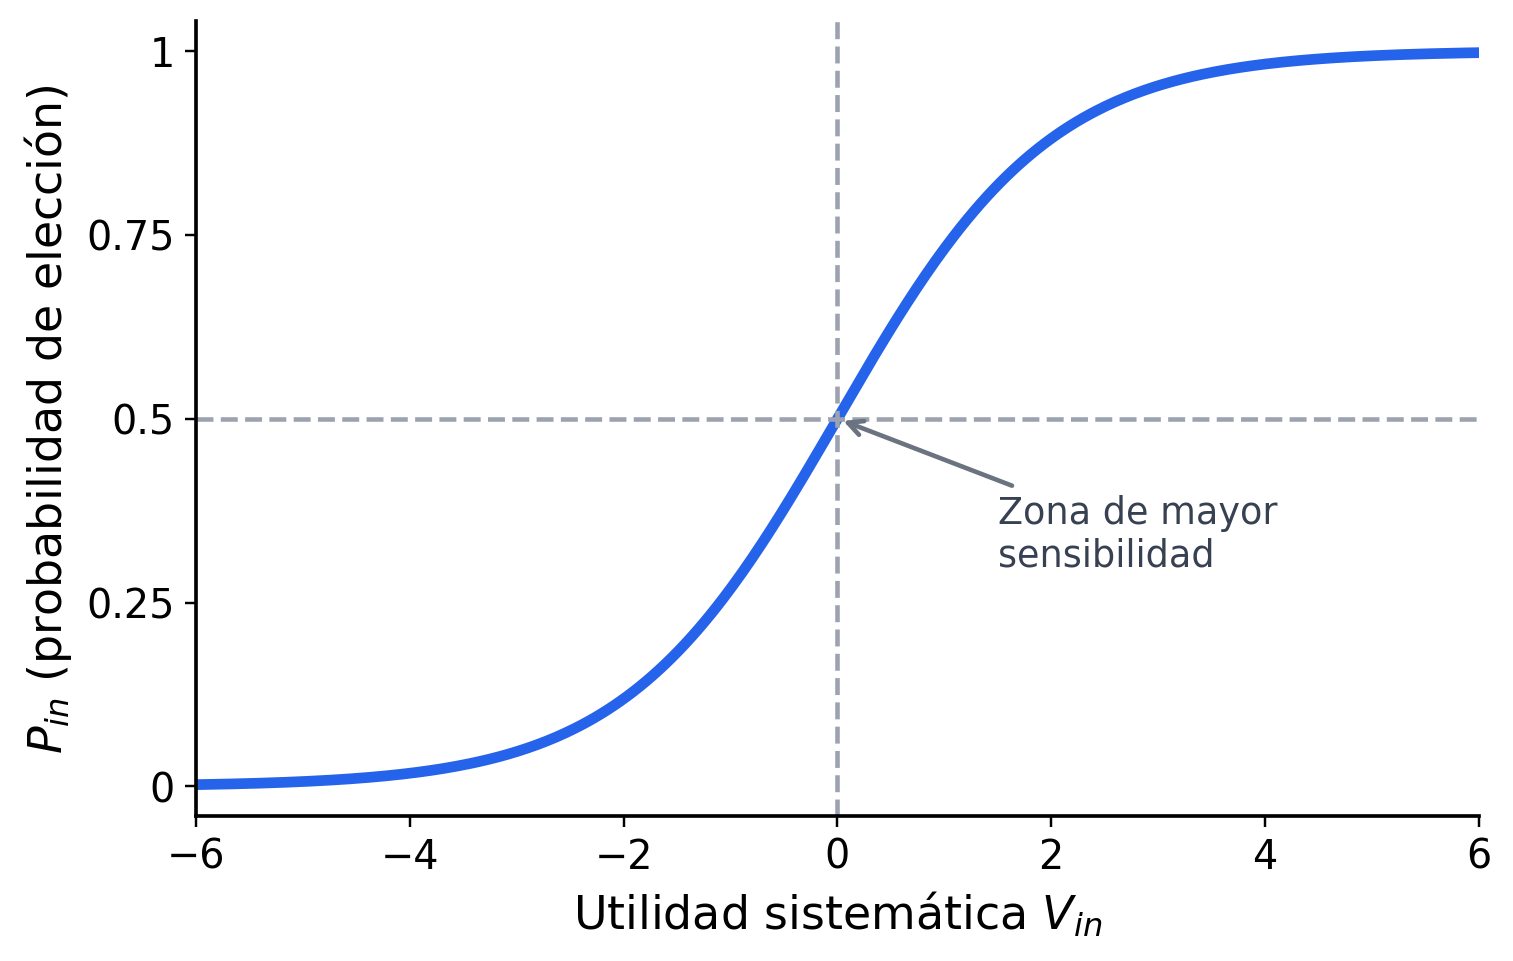
\includegraphics[width=0.5\textwidth]{figs/mnl_sigmoid.png}
    \caption{Forma sigmoidal ilustrativa de la probabilidad de elección en el modelo \gls{mnl}. Elaboración propia con Python y Matplotlib.}
    \label{fig:mnl_sigmoid}
\end{figure}
\newpage

En la práctica, la componente determinista de la utilidad suele especificarse como una combinación lineal de atributos observables:\newline
\begin{equation}
V_{in} = \beta_{i0} + \sum_{k}\beta_{ik}x_{ink}
\end{equation}
\newline
donde $x_{ink}$ representa el valor del atributo $k$ asociado a la alternativa $i$ para el individuo $n$, $\beta_{ik}$ es el parámetro que mide la influencia de dicho atributo y $\beta_{i0}$ es una constante específica de la alternativa. Esta formulación permite cuantificar el efecto relativo de variables como el tiempo de viaje, el coste monetario, el número de transbordos o el acceso peatonal, entre otras. En términos interpretativos, los parámetros estimados indican cómo varía la utilidad de cada modo cuando cambian sus atributos observables.\newline

La estimación de los parámetros del modelo se realiza habitualmente mediante máxima verosimilitud. Para ello, se define una función de verosimilitud que mide la probabilidad de observar las elecciones registradas en la muestra dadas unas determinadas estimaciones de los parámetros. El objetivo del proceso de ajuste consiste en encontrar los valores de $\beta$ que maximizan dicha verosimilitud, o de forma equivalente, que maximizan la log-verosimilitud del modelo. Este procedimiento constituye la base clásica de estimación de modelos de elección discreta y permite obtener un modelo interpretable y coherente con la teoría del comportamiento del viajero.\newline

En este TFM, el modelo \gls{mnl} resulta relevante como referencia metodológica, ya que proporciona una base teórica sólida para representar la elección modal a partir de atributos del desplazamiento. Además, sirve como punto de comparación frente a enfoques más flexibles basados en aprendizaje automático, que se describen en los apartados siguientes.\newline

Una limitación conocida del modelo \gls{mnl} es la hipótesis de \gls{iia}, derivada de la suposición de errores independientes e idénticamente distribuidos. Esta propiedad implica que la relación de sustitución entre dos alternativas no depende de la presencia o de las características del resto de modos, lo cual puede resultar restrictivo en problemas de movilidad donde algunas opciones están más correlacionadas entre sí que otras \cite{McFadden1974,Train2009}. Aun así, el \gls{mnl} sigue siendo el punto de partida más habitual en la literatura por su equilibrio entre simplicidad, interpretabilidad y capacidad descriptiva.



\subsection{Limitaciones del enfoque clásico}

A pesar de su amplia utilización en el análisis de elección modal, los modelos basados en utilidad aleatoria presentan ciertas limitaciones cuando se aplican a problemas complejos de movilidad. En primer lugar, requieren especificar de forma explícita la forma funcional de la utilidad sistemática, lo que implica que el analista debe decidir previamente qué variables incluir y cómo se relacionan con la utilidad de cada alternativa. En muchos casos, esta especificación se realiza mediante combinaciones lineales de atributos del viaje, lo que puede resultar restrictivo cuando las relaciones reales entre variables son no lineales o presentan interacciones complejas \cite[p.~20]{MartinBaos2023Thesis}.\newline

Otra limitación relevante es que los modelos clásicos suelen asumir estructuras relativamente simples en la distribución de los términos de error. En el caso del \acrlong{mnl}, por ejemplo, la hipótesis de \acrlong{iia} puede no reflejar adecuadamente situaciones en las que algunas alternativas presentan correlaciones más fuertes entre sí, como ocurre frecuentemente entre distintos modos de transporte público o entre modos motorizados.\newline

Además, desde un punto de vista práctico, la especificación de modelos econométricos puede requerir un proceso iterativo de selección de variables, transformación de atributos y validación de supuestos teóricos. Aunque este enfoque proporciona modelos interpretables y coherentes con la teoría del comportamiento del viajero, puede resultar menos flexible cuando se trabaja con conjuntos de datos de alta dimensionalidad o con relaciones complejas entre variables.


\subsection{Aprendizaje automático para elección modal}

Con el aumento de la disponibilidad de datos y de la capacidad computacional, en los últimos años han ganado relevancia los enfoques basados en aprendizaje automático para el análisis de elección modal. Desde esta perspectiva, la elección de modo puede formularse también como un problema de clasificación supervisada, en el que el objetivo consiste en predecir la alternativa elegida a partir de un conjunto de variables explicativas relacionadas con el viaje y con las características del individuo.
\newpage

A diferencia de los modelos clásicos de elección discreta, muchos algoritmos de aprendizaje automático no requieren especificar de forma explícita la forma funcional de la relación entre variables. En su lugar, aprenden patrones directamente a partir de los datos de entrenamiento, lo que les permite capturar relaciones no lineales, interacciones complejas entre atributos y estructuras de decisión difíciles de representar mediante modelos lineales tradicionales.\newline

Entre las técnicas más utilizadas en este contexto destacan los métodos basados en árboles de decisión y los modelos de conjunto (\textit{ensemble models}) derivados de ellos, como \acrlong{rf} o \acrlong{gbdt}, así como los modelos basados en \glspl{dnn}. Estos enfoques han mostrado un rendimiento predictivo competitivo en numerosos problemas de clasificación tabular, incluyendo aplicaciones en transporte y elección modal.\newline

En este trabajo se adopta esta perspectiva complementaria: el \acrlong{mnl} se considera como referencia metodológica clásica, mientras que distintos modelos de aprendizaje automático se utilizan para explorar alternativas con mayor capacidad predictiva. En particular, la arquitectura del simulador se ha diseñado para permitir la integración de diferentes modelos de clasificación como \gls{rf}, \acrshort{xgboost} y \glspl{dnn}, de forma que puedan compararse sus resultados en el contexto del problema de elección modal analizado. Esta comparación resulta coherente con la evidencia reciente disponible para datasets reales de elección modal, entre ellos \gls{lpmc} \cite{Hillel2018LPMC}.\newline

\subsection{Random Forests}

Random Forest es un método de aprendizaje automático basado en la combinación de múltiples árboles de decisión entrenados sobre subconjuntos distintos de los datos. El modelo fue propuesto por Breiman \cite{Breiman2001} como una extensión de los árboles de clasificación tradicionales, con el objetivo de mejorar su estabilidad y capacidad predictiva. En diversas revisiones de la literatura, este tipo de modelos aparece además como una de las familias más utilizadas en comparativas recientes de elección modal.
\newpage

La idea fundamental consiste en entrenar un gran número de árboles de decisión sobre diferentes subconjuntos de los datos de entrenamiento. Cada árbol se construye utilizando una muestra aleatoria del conjunto de datos original (técnica conocida como \textit{bootstrap sampling}) y, además, en cada división del árbol se considera únicamente un subconjunto aleatorio de variables explicativas. Este doble proceso de aleatorización permite reducir la correlación entre árboles individuales y, en consecuencia, mejorar el rendimiento del modelo agregado.\newline

En problemas de clasificación, como el de elección modal, cada árbol produce una predicción independiente y la decisión final se obtiene mediante votación mayoritaria entre todos los árboles del bosque. Este mecanismo permite capturar relaciones no lineales entre variables y manejar de forma robusta conjuntos de datos con múltiples atributos.\newline

En el ámbito del transporte, los modelos \acrlong{rf} se han utilizado en distintos trabajos para predecir la elección de modo de transporte, ya que ofrecen un buen equilibrio entre capacidad predictiva, robustez frente al sobreajuste y relativa facilidad de interpretación mediante medidas de importancia de variables. No obstante, la evidencia comparativa reciente sugiere que su rendimiento puede quedar por debajo del de otros métodos más potentes de boosting en algunos conjuntos de datos reales \cite{MartinBaos2023TRC}.

\subsection{Gradient Boosting Decision Trees}

Los modelos basados en \gls{gbdt} constituyen otra familia de métodos de aprendizaje automático ampliamente utilizados en problemas de clasificación con datos tabulares. A diferencia de los métodos basados en bagging, como \acrlong{rf}, el enfoque de boosting construye los árboles de decisión de forma secuencial, de modo que cada nuevo árbol intenta corregir los errores cometidos por el conjunto de árboles anteriores \cite{Friedman2001}.\newline

El proceso comienza entrenando un primer árbol de decisión sencillo sobre los datos de entrenamiento. A continuación, se construyen árboles adicionales que se ajustan sobre los residuos o errores del modelo previo. De este modo, el modelo final se obtiene como la suma ponderada de múltiples árboles débiles, cada uno de los cuales contribuye a mejorar gradualmente la predicción global.
\newpage

Entre las implementaciones más conocidas de este enfoque se encuentra \gls{xgboost}, una biblioteca optimizada que introduce mejoras en eficiencia computacional, regularización del modelo y manejo de grandes conjuntos de datos \cite{Chen2016XGBoost}. Gracias a estas características, \gls{xgboost} se ha convertido en una de las técnicas más utilizadas en problemas de aprendizaje supervisado con datos estructurados y ha mostrado un comportamiento especialmente competitivo en comparativas recientes de elección modal.\newline

En el contexto de este TFM, los modelos basados en \textit{Gradient Boosting} cobran relevancia, ya que permiten capturar relaciones no lineales entre los atributos del viaje y la elección modal. Además, su buen rendimiento predictivo y su flexibilidad para manejar distintos tipos de variables los convierten en una herramienta adecuada para integrarse en el simulador de movilidad desarrollado en este trabajo.

\subsection{Redes Neuronales Profundas}

Las \glspl{dnn} constituyen otra familia de modelos de aprendizaje automático que ha experimentado un crecimiento significativo en los últimos años. Estas técnicas se basan en arquitecturas formadas por múltiples capas de neuronas artificiales que transforman progresivamente las variables de entrada mediante combinaciones lineales y funciones de activación no lineales \cite{Goodfellow2016}.\newline

A diferencia de los modelos basados en árboles, las redes neuronales permiten aprender representaciones internas de los datos a través de varias capas ocultas, lo que facilita capturar relaciones complejas entre variables. Esta capacidad de modelar interacciones no lineales ha motivado su aplicación en numerosos problemas de predicción y clasificación, incluyendo el análisis del comportamiento de los viajeros.\newline

En problemas de elección modal, las redes neuronales profundas pueden utilizarse para estimar la probabilidad de seleccionar cada modo de transporte a partir de atributos del desplazamiento y características sociodemográficas del usuario. Aunque estos modelos suelen requerir mayor volumen de datos y un proceso de ajuste más cuidadoso que los métodos basados en árboles, también ofrecen una elevada flexibilidad para capturar patrones complejos presentes en los datos.\newline

% Los tres enfoques descritos en esta sección (\gls{rf}, \gls{xgboost}, \gls{dnn}) se evalúan de forma comparativa sobre el dataset \gls{lpmc}. Su entrenamiento, ajuste e integración en el simulador de movilidad se detallan en el Capítulo~\ref{ch:implementacion}.